\newcommand{\ClassPath}{../VIU_TFM_LaTeX_template}
\documentclass{\ClassPath/viu-tfm-template}
\usepackage{multicol}

\definecolor{maincolor}{HTML}{f25416}

%--------------------------------------------------------------------------
% Definiciones necesarias Modifica con tus datos
%--------------------------------------------------------------------------
\def\nombre{Gómez Olivencia, Rubén}
\def\dni{78910013-A}
\def\titulo{Análisis de vulnerabilidades \linebreak\linebreak de un portal web}
\def\titulacion{Máster Universitario en Desarrollo de Aplicaciones y Servicios Web}
\def\curso{2022-2023}

%Los siguientes son opcionales: si no se ponen, la portada cambia un poco. Ideal para escribir artículos/trabajos cortos
\def\dirige{}
\def\convocatoria{}
\def\asignatura{Seguridad Web}


% importar fichero de Bibliografía
%\addbibresource{Actividad_1.bib}

\begin{document}


\graphicspath{{../VIU_TFM_LaTeX_template/}}

\coverpage

\tableofcontents

\chapter{Introducción}

La seguridad en un proyecto informático es algo que se debe pensar desde el inicio del mismo, ya que las decisiones tomadas pueden repercutir en las iteraciones posteriores y en la evolución del producto que estemos realizado.

Hoy en día es habitual hacer uso de \textit{frameworks} a la hora de facilitar la programación de una aplicación web. Gracias a ello nos va a permitir hacer uso de buenas prácticas, que junto con el funcionamiento interno del \textit{framework} van a evitar que tengamos ciertos fallos de seguridad habituales como puede ser el \textbf{\textit{SQL injection}}.

Eso no quita que debamos de realizar un análisis de la aplicación que estamos desarrollando, tratando de buscar posibles vulnerabilidades antes de que el proyecto salga a producción.

A lo largo de este documento se van a utilizar distintas herramientas de análisis que van a ser ejecutadas contra la web \href{http://testphp.vulnweb.com/}{http://testphp.vulnweb.com/}, ya que es un portal creado especialmente con vulnerabilidades con el propósito de ser analizado y aprender en el proceso.


\chapter{Objetivo}
El objetivo de este documento es el de aprender a utilizar ciertas herramientas que nos van a permitir realizar un análisis de un portal web para tratar de buscar las vulnerabilidades más habituales que nos encontramos hoy en día en el ámbito web:

\begin{itemize}
    \item \textbf{Inyección de SQL} (“\textit{SQL injection}” en inglés): Es una vulnerabilidad causada por no comprobar (o no hacerlo de  manera correcta) los valores de una variable que posteriormente es utilizada de forma incorrecta para realizar una sentencia SQL. De esta manera, se “inyecta” código que puede permitir realizar acciones sobre la base de datos que no deberían estar permitidas (obtener datos confidenciales, borrar datos, ...).

    \item \textbf{\textit{Cross-site Scripting}} (\textbf{XSS}): En castellano “secuencia de comandos en sitios cruzados”, que significa que un atacante puede inyectar código javascript en ficheros del servidor. También permite obtener información como sesiones de usuarios o comprometer el navegador del visitante.

    \item \textbf{\textit{Cross-site Request Forgery}} (\textbf{CSRF}): En castellano “falsificación de petición en sitios cruzados”, que se refiere a un tipo de  vulnerabilidad en el que un portal web ejecuta comandos no autorizados por ser transmitidos por un usuario desde el cual el sitio web confía.
\end{itemize}

Tal como se ha dicho previamente, el análisis va a ser realizado contra el portal web \href{http://testphp.vulnweb.com/}{http://testphp.vulnweb.com/}, aunque podríamos utilizar un desarrollo propio que estemos realizando.

No sería ético realizar un análisis de un portal ajeno tratando de buscar vulnerabilidades que podamos atacar en nuestro propio beneficio.


\chapter{Análisis general}

Aunque alguna de las vulnerabilidades previamente descritas podrían ser fácilmente detectadas haciendo uso del método “prueba-error”, es más interesante hacer uso de herramientas que nos pueden realizar un informe tratando de buscar las vulnerabilidades más habituales.

Una de estas herramientas es \href{https://www.arachni-scanner.com/}{Arachni Scanner}, que nos va a realizar un rastreo de todo el portal web que le indiquemos, realizando distintas comprobaciones y finalmente realizando un informe detallando todas las vulnerabilidades encontradas.

\section{Arachni Scanner}
\href{https://www.arachni-scanner.com/}{Arachni} permite ser usado a través de línea de comandos o desde un interfaz web propio que levanta con su propio servidor web haciendo uso del comando \commandbox{./arachni_web} que se tiene que ejecutar desde el directorio creado tras realizar la \href{https://www.arachni-scanner.com/download/}{descarga}.

La herramienta permite crear distintos perfiles con los que realizar los análisis que más nos interesen. Por defecto trae tres perfiles ya creados:

\begin{itemize}
    \item \textbf{Default}: Perfil por defecto que va a realizar un análisis profundo tratando de buscar todo tipo de vulnerabilidades.

    También va a realizar la búsqueda de ficheros o directorios de backups (que en caso de ser descargados podrían contener datos privados y/o código fuente), ficheros con información sensible, interfaces de administración que deberían estar ocultas...

    Es un análisis complejo que va a necesitar bastante tiempo, pero nos va a dar como resultado un informe muy detallado.

    \item \textbf{SQL injection}: Perfil que sólo va a tratar de obtener las vulnerabilidades relacionadas con \textit{SQL injection}.

    \item \textbf{Cross-Site Scripting (XSS)}: Como el caso anterior, pero esta vez obteniendo las vulnerabilidades XSS.
\end{itemize}

\section{Informe obtenido}

Para la realización de este documento se ha utilizado el perfil “\textit{default}” para tratar de buscar todas las vulnerabilidades posibles del portal.

Esto ha hecho que el análisis haya tardado un total de 45 minutos y 37 segundos, pero que ha permitido obtener un total de 173 vulnerabilidades, que Arachni diferencia de la siguiente forma.

{
    \hfill
    \begin{minipage}{0.4\linewidth}
        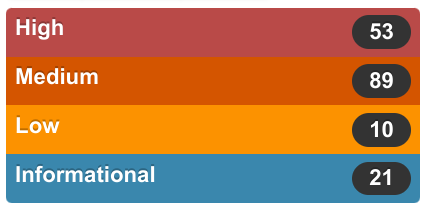
\includegraphics[width=\linewidth]{img/total.png}
    \end{minipage}
    \hfill
    \hfill
    \begin{minipage}{0.3\linewidth}
        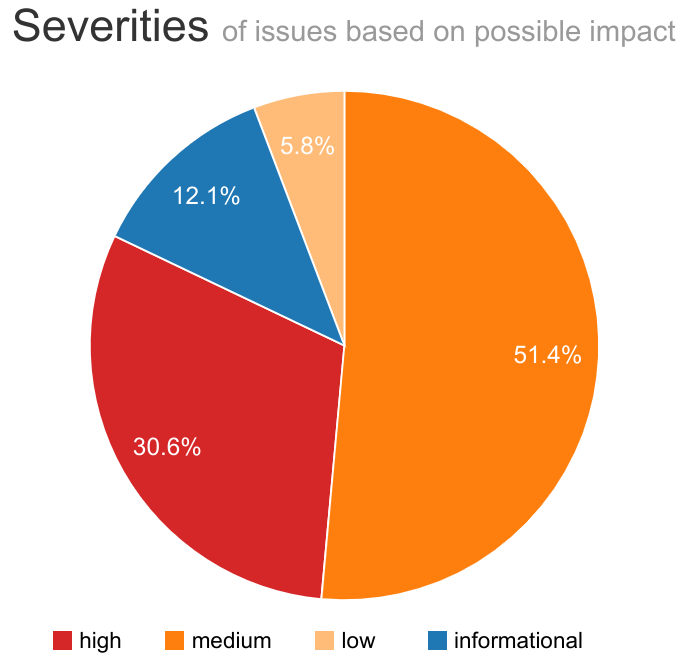
\includegraphics[width=\linewidth]{img/grafico.png}
    \end{minipage}
    \hfill
}

Tal como se puede ver, el número de vulnerabilidades de medio y alto riesgo suponen un gran porcentaje de las obtenidas, por lo que a simple vista se puede asumir que el portal corre riesgo severo en su seguridad.

Si entramos al listado detallado, Arachni nos las diferencia de la siguiente manera:

\begin{center}
    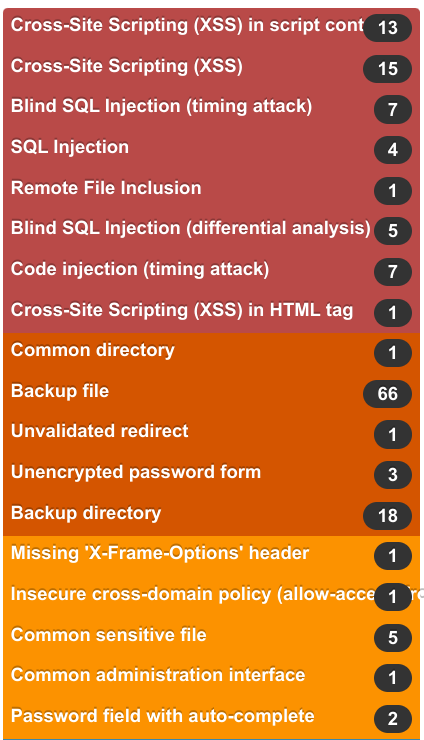
\includegraphics[width=0.5\linewidth]{img/lista.png}
\end{center}
\vspace{-20pt}

Para cada uno de estas vulnerabilidades Arachni genera una página detallada con el ataque realizado y la prueba obtenida.

\hypertarget{vulnerabilidad_xss}{}
\chapter{Vulnerabilidades XSS}
Para el caso de vulnerabilidades \textit{Cross-Site Scripting} (\textbf{XSS}). En la siguiente imagen se puede ver parte del listado junto con las URLs del portal.

\begin{center}
    \vspace{-9pt}
    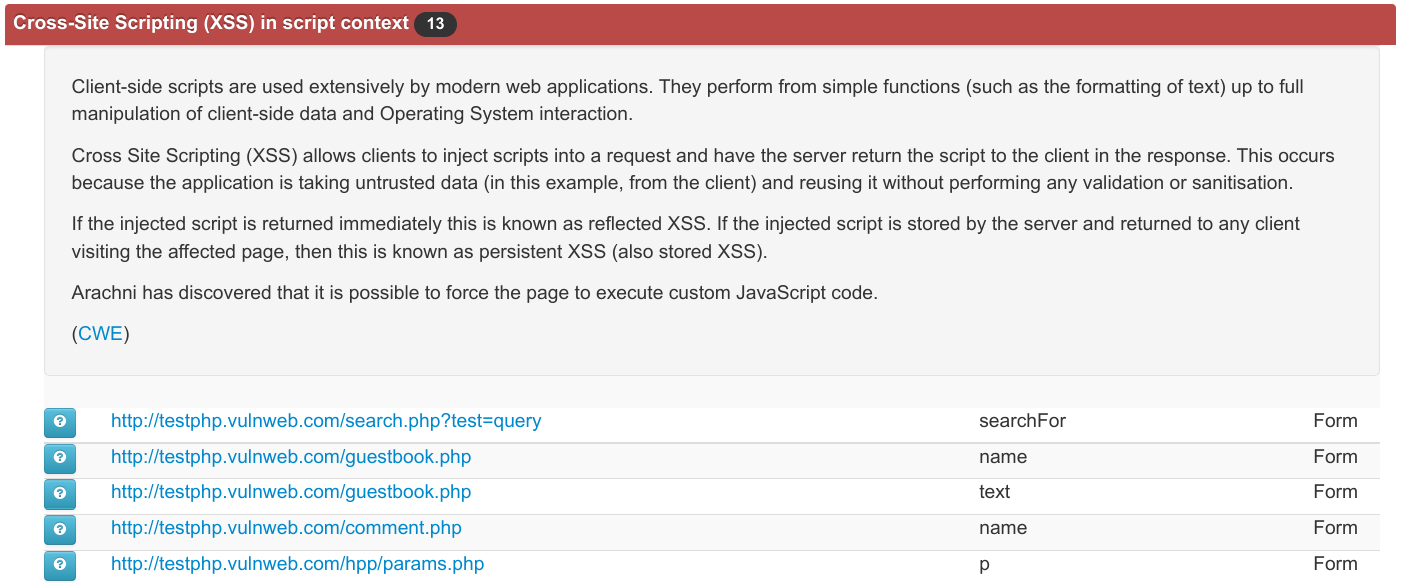
\includegraphics[frame,width=0.8\linewidth]{img/lista_xss.png}
\end{center}

Si se hace click en algún icono de la izquierda del listado, nos llevará al informe detallado de la vulnerabilidad elegida. Por ejemplo, en el caso de la URL \href{http://testphp.vulnweb.com/guestbook.php}{http://testphp.vulnweb.com/guestbook.php} nos indica la prueba realizada y el resultado de la misma, dando en este caso como resultado que es vulnerable:

\begin{center}
    \vspace{-10pt}
    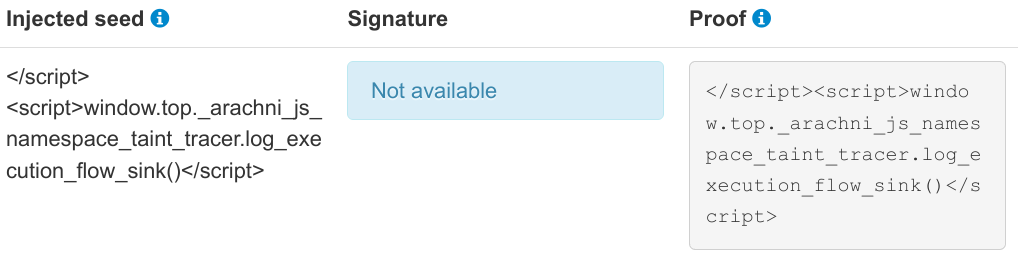
\includegraphics[frame,width=0.9\linewidth]{img/informe_xss.png}
\end{center}

Lo que ha hecho de manera automatizada Arachni es meter un javascript en un formulario que aparece en la mencionada URL, para luego comprobar si ese código aparece en el HTML generado.

Si realizamos la misma prueba, pero haciendo algo más evidente, como el siguiente código:

\begin{mycode}{Ejemplo de Cross-Site Scripting}{html}{}
</script><script>alert('hacked')</script>
\end{mycode}

Obtendremos que la web ha insertado el código en el HTML, y en este caso ejecuta el script introducido:


\begin{center}
    \vspace{-10pt}
    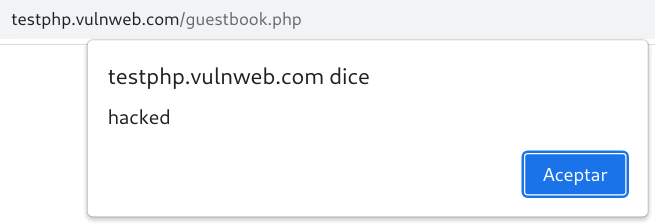
\includegraphics[width=0.7\linewidth]{img/ejemplo_xss.png}
\end{center}
\vspace{-10pt}



\chapter{Vulnerabilidades SQL injection}
Para el caso de las \textit{SQL Injection}, Arachni nos ha encontrado 4 vulnerabilidades en varias URLs. Para profundizar en este tipo de vulnerabilidades vamos hacer uso de \href{https://sqlmap.org/}{SQLmap}, que es una herramienta de consola que nos va a permitir obtener información de la base de datos a través de estos fallos.

Como ejemplo, se va a utilizar una de las URLs del informe de Arachni: \href{http://testphp.vulnweb.com/listproducts.php?cat=1}{http://testphp.vulnweb.com/listproducts.php?cat=1}. En este caso SQLmap es una herramienta de consola a la que pasamos la URL elegida.

\begin{mycode}{Obtención de información con SQLmap}{console}{}
ruben@vega:/tmp/sqlmap-dev$ ./sqlmap.py \
-u "http://testphp.vulnweb.com/listproducts.php?cat=1" --batch
...
[20:47:32] [INFO] the back-end DBMS is MySQL
web server operating system: Linux Ubuntu
web application technology: Nginx 1.19.0, PHP 5.6.40
back-end DBMS: MySQL >= 5.6


ruben@vega:/tmp/sqlmap-dev$ ./sqlmap.py \
-u "http://testphp.vulnweb.com/listproducts.php?cat=1" \
--batch --dbs
...
available databases [2]:
[*] acuart
[*] information_schema

ruben@vega:/tmp/sqlmap-dev$ ./sqlmap.py \
-u  "http://testphp.vulnweb.com/listproducts.php?cat=1" \
--batch --tables -D acuart
...
Database: acuart
[8 tables]
+-----------+
| artists   |
| carts     |
| categ     |
| featured  |
| guestbook |
| pictures  |
| products  |
| users     |
+-----------+
\end{mycode}

Tal como se puede ver, gracias a SQLmap se ha obtenido la versión del gestor de bases de datos (MySQL 5.6 o superior), y con otros comandos se ha podido obtener el nombre de la base de datos y las tablas que contiene.

SQLmap nos permite hacer mucho más a través de distintos parámetros, como es obtener información del usuario que realiza las peticiones, o incluso poder realizar un volcado de todas las bases de datos a las que se tiene acceso.


\chapter{Vulnerabilidades CSRF}
Aunque Arachni también es capaz de buscar vulnerabilidades CSRF, no nos ha detectado ninguna en este caso. Es por eso que se ha hecho uso de \href{https://github.com/s0md3v/Bolt}{Bolt}, que es un escaneador específico para vulnerabildiades CSRF, para confirmar si existe alguna vulneravilidad o no.

Es una aplicación de consola hecha en \href{https://www.python.org/}{Python}, que nos va a permitir obtener las URLs que contienen formularios inseguros.

\begin{mycode}{Buscando vulnerabilidades CSRF con Bolt}{console}{{\small }}
ruben@vega:/tmp/Bolt$ python3 bolt.py \
-u  http://testphp.vulnweb.com/ -l 10 -t 10
⚡ Phase: Crawling [1/6]
[!] Crawled 13148 URL(s) and found 13148 form(s).
⚡ Phase: Evaluating [2/6]
[-] http://testphp.vulnweb.com/ [search.php?test=query]
[-] http://testphp.vulnweb.com/login.php [userinfo.php]
[-] http://testphp.vulnweb.com/login.php [search.php?test=query]
[-] http://testphp.vulnweb.com/cart.php [search.php?test=query]
[-] http://testphp.vulnweb.com/categories.php [search.php?test=query]
[-] http://testphp.vulnweb.com/index.php [search.php?test=query]
[-] http://testphp.vulnweb.com/guestbook.php [search.php?test=query]
[-] http://testphp.vulnweb.com/disclaimer.php [search.php?test=query]
[-] http://testphp.vulnweb.com/userinfo.php [userinfo.php]
[-] http://testphp.vulnweb.com/userinfo.php [search.php?test=query]
[-] http://testphp.vulnweb.com/artists.php [search.php?test=query]
[-] http://testphp.vulnweb.com/signup.php [secured/newuser.php]
[-] http://testphp.vulnweb.com/signup.php [search.php?test=query]
[-] http://testphp.vulnweb.com/artists.php [search.php?test=query]
[-] http://testphp.vulnweb.com/listproducts.php [search.php?test=query]
[-] http://testphp.vulnweb.com/listproducts.php [search.php?test=query]
[-] http://testphp.vulnweb.com/artists.php [search.php?test=query]
[-] http://testphp.vulnweb.com/listproducts.php [search.php?test=query]
[-] http://testphp.vulnweb.com/listproducts.php [search.php?test=query]
[-] http://testphp.vulnweb.com/artists.php [search.php?test=query]
...
\end{mycode}

Tal como se puede ver, Bolt ha realizado sus pruebas y ha encontrado varios formularios que son vulnerables a ataques CSRF.


\chapter{Posibles soluciones a realizar}
Para realizar un buen informe de vulnerabilidades detectadas, no sólo hay que nombrarlas, sino que hay que tratar de aportar información y posibles maneras para resolverlas.

Lo ideal sería hacer un estudio del código fuente de la aplicación para cada una de las vulnerabilidades detectadas, así como de la configuración del servidor donde se encuentra. De esta manera, se podría otorgar soluciones más precisas, ya que para cada vulnerabilidad pueden existir distintas posibles soluciones.

A continuación se detallan algunas de las posibles soluciones para corregir parte de las vulnerabilidades encontradas.

\section{Corregir vulnerabilidades XSS}
Debido a cómo funcionan las vulnerabilidades XSS, en las que mayormente es un ataque a través de cajas de texto (ya sea en formularios, páginas de búsqueda, inserción de comentarios ...) la primera solución a efectuar es comprobar el texto que recibimos en el \textit{backend}.

Existen distintas maneras de realizar dicha comprobación, pero alguna de ellas podría ser:

\begin{itemize}
    \item \textbf{Escapar caracteres}: Debido a que algunos caracteres introducidos pueden utilizarse como vector de ataque (tal como hemos visto \hyperlink{vulnerabilidad_xss}{previamente} con los “</script>”), la idea es convertir esos caracteres a formato html, o “escapando” dichos caracteres.

    \item \textbf{Eliminar caracteres no permitidos:} Una alternativa más radical a la anterior sería directamente eliminar todo carácter no permitido cuando un formulario es enviado.
\end{itemize}

A cualquiera de estas formas  se le suele denominar “\textbf{\textit{sanitize}}” en inglés, y hoy en día existen plugins (o los propios \textit{frameworks} traen funciones) que permiten realizar estas funciones de manera automática.

Por supuesto, los lenguajes de programación (sobre todo los orientados a la web) también traen sus propias funciones. Y de no ser así, siempre podríamos crearnos una función propia añadiendo los caracteres que nos interese eliminar para que sean sustituidos.


\section{Corregir vulnerabilidades SQL injection}

Similar al caso anterior, las \textbf{\textit{SQL injection}} funcionan debido al código que se pasa a través de formularios que permiten ejecutar sentencias SQL que no deberían permitirse.

Por lo tanto, la primera solución debería ser la misma que en el caso anterior, no permitir caracteres que puedan alterar la sentencia SQL que se van a ejecutar desde el código fuente.

Por otro lado, lo ideal es hacer uso del sistema de parametrización de sentencias SQL que suelen tener los frameworks actuales, ya que se encargan de realizar las funciones necesarias para evitar este tipo de ataques.

En el caso del \textit{framework} \href{https://laravel.com/}{Laravel}, cuenta con el sistema \href{https://laravel.com/docs/6.x/eloquent}{Eloquent} que es el \textbf{ORM} (\textit{object–relational mapping} o asignación objeto-relacional) que viene incluído. De esta manera, antes de ejecutar la correspondiente sentencia SQL convertirá los datos al sistema esperado por la base de datos objeto. En caso de que la conversión de datos no sea correcta, habrá un error y por tanto la sentencia no será ejecutada.


Por último, también existe la posibilidad de tener distintos usuarios de base de datos para una misma aplicación, limitando las acciones que puede realizar cada usuario a nivel de sistema gestor de base de datos. Esta solución puede ser más compleja, y dependerá de la aplicación que estemos realizando, pero es conveniente tenerla en cuenta.


\section{Corregir vulnerabilidades CSRF}
Este tipo de ataques también se forma en los formularios, por lo que la manera en la que lo podemos corregir es añadiendo un \textit{\textbf{token CSRF}} que debe cumplir lo siguiente:

\begin{itemize}
    \item Debe ser \textbf{único por sesión}.
    \item Debe ser secreto la manera en la que se genera.
    \item \textbf{Impredicible}. Debe tener una buena longitud y que sea generado por un método seguro.
\end{itemize}

De nuevo nos podemos basar en las buenas prácticas de los \textit{framewors} para mitigar este tipo de ataques, ya que hoy en día cuentan con la generación de estos tokens de manera automatizada.

En el caso de Laravel, en la documentación oficial se \href{https://laravel.com/docs/6.x/csrf}{explica cómo podemos adaptar nuestro código} incluyendo una directiva en nuestros formularios que generará el token.

\begin{mycode}{Añadir token CSRF en Laravel}{html}{}
<form method="POST" action="/profile">
    @csrf
    ...
</form>
\end{mycode}

Tal como se puede ver, con una línea tan sencilla conseguimos evitar este tipo de vulnerabilidades.

%Añadido a esto, y para mejorar la protección, también podemos realizar configuraciones en la parte del servidor web para limitar el origen de las peticiones. Podríamos crear una


\chapter{Conclusiones}

A la hora de crear nuestros proyectos web es importante conocer los distintos tipos de vulnerabilidades existentes para tratar de no cometer los fallos que generen dichas vulnerabilidades.

Como somos humanos, y cometemos errores, es importante conocer distintos sistemas capaces de encontrar  estas vulnerabilidades para que podamos corregirlas antes de pasar nuestra aplicación a producción.

Interiorizar estos conocimientos, hacer uso de buenas prácticas y utilizar las distintas herramientas que nos proveen los \textit{frameworks} no va a evitar que realicemos errores en nuestro código, pero mejorará la seguridad y nos ayudará a prevenir las vulnerabilidades más habituales.

\end{document}